\documentclass{book}
\usepackage[margin=3cm]{geometry}

\usepackage{uninafrontespizio}
\usepackage[italian]{babel}
\usepackage{svg}

\Universita{Università degli Studi di Napoli Federico II}
\Facolta{Scuola Politecnica e delle Scienze di Base}
\Dipartimento{Dipartimento di Ingegneria Elettrica e Tecnologie dell'Informazione}
\CorsoDiLaurea{Corso di Laurea Triennale in Informatica}
\Materia{Progetto di Ingegneria del Software}
\AnnoAccademico{Anno Accademico 2024--2025}
\Titolo{DietiEstates25}
\Studente{Fabrizio Apuzzo}
\Studente{Maria Della Valle}
\StudenteLabel{Studenti}
\Professore{Sergio Di Martino}
\Professore{Luigi Libero Lucio Starace}
\ProfessoreLabel{Professori}
\Logo{figures/logo-federico-II.pdf}
\LogoWidth{3.5cm}
\LogoPosition{below-uni}

\begin{document}

\pagestyle{empty}
\makefrontpage
\pagestyle{headings}
\tableofcontents
\setcounter{chapter}{-1}

\chapter{Introduzione}

\textbf{DietiEstates25} è una piattaforma dedicata alla gestione di servizi immobiliari che consente alle agenzie di pubblicare annunci di proprietà ed agli utenti di visualizzare gli immobili disponibili ed effettuare offerte di acquisto o locazione.\\\\
Il presente documento illustra dettagliatamente il processo di sviluppo del sistema DietiEstates25 dall'analisi dei requisiti, alle scelte progettuali, per concludersi con i test di verifica all'implementazione e con la valutazione dell'usabilità della piattaforma.

\section{Struttura del Documento}

Il documento è organizzato in tre capitoli che seguono il processo di sviluppo del sistema DietiEstates25:

\begin{itemize}
    \item Il \textbf{Capitolo 1 - Analisi e Specifica dei Requisiti Software} presenta un'analisi delle funzionalità del sistema attraverso diagrammi UML, descrizioni testuali strutturate secondo i template di A. Cockburn e prototipi delle interfacce utente. Include inoltre una definizione degli utenti target e modelli di dominio per la formalizzazione del problema.

    \item Il \textbf{Capitolo 2 - Progettazione del Sistema} illustra le scelte architetturali e le tecnologiche adottate, con l'ausilio di notazioni UML. Particolare attenzione è dedicata alla progettazione delle interfacce utente e alla motivazione delle scelte progettuali effettuate.

    \item Il \textbf{Capitolo 3 - Testing e Valutazione dell'Usabilità} presenta la fase di verifica del sistema attraverso test automatici. Include inoltre una valutazione dell'usabilità condotta mediante ispezioni sistematiche e test con utenti reali, completata da un'analisi dei risultati dei questionari di valutazione.
\end{itemize}

\chapter{Analisi e Specifica dei Requisiti Software}

Il primo passo per la creazione del sistema DietiEstates25 è l'identificazione dei requisiti con successiva analiisi. Quest'ultima è strutturata partendo dalla definizione degli utenti target. Segue la modellazione dei casi d'uso con l'ausilio di Use Case Diagram, descrizioni testuali e prototipi rapidi di interfacce utente.

\section{Individuazione dei Target}

Un sistema di annunci immobiliari come DietiEstates25 può avere come target diversi gruppi di utenti. Sono state identificate però tre distinte categorie principali, ognuna con specifiche necessità e livelli di accesso alle funzionalità della piattaforma:
\begin{itemize}
    \item Clienti
    \item Agenti immobiliari
    \item Amministratori
\end{itemize}
Segue una definizione di ciascuno di essi, accompagnata da esempi di utenti tipici di ognuna delle categorie, illustrati tramite \textit{Personas}.

\subsection{Clienti}
Utilizzatori principali dei servizi offerti da DietiEstates25, i clienti si configurano come il gruppo più ampio degli utenti. Si tratta di soggetti interessati all'acquisto di immobili, motivati dall'opportunità di ottenere prezzi vantaggiosi tramite il sistema di offerte. Possono appartenere a qualsiasi fascia di età o classe economica e ognuno ha esigenze differenti.

\begin{figure}[!htb]
    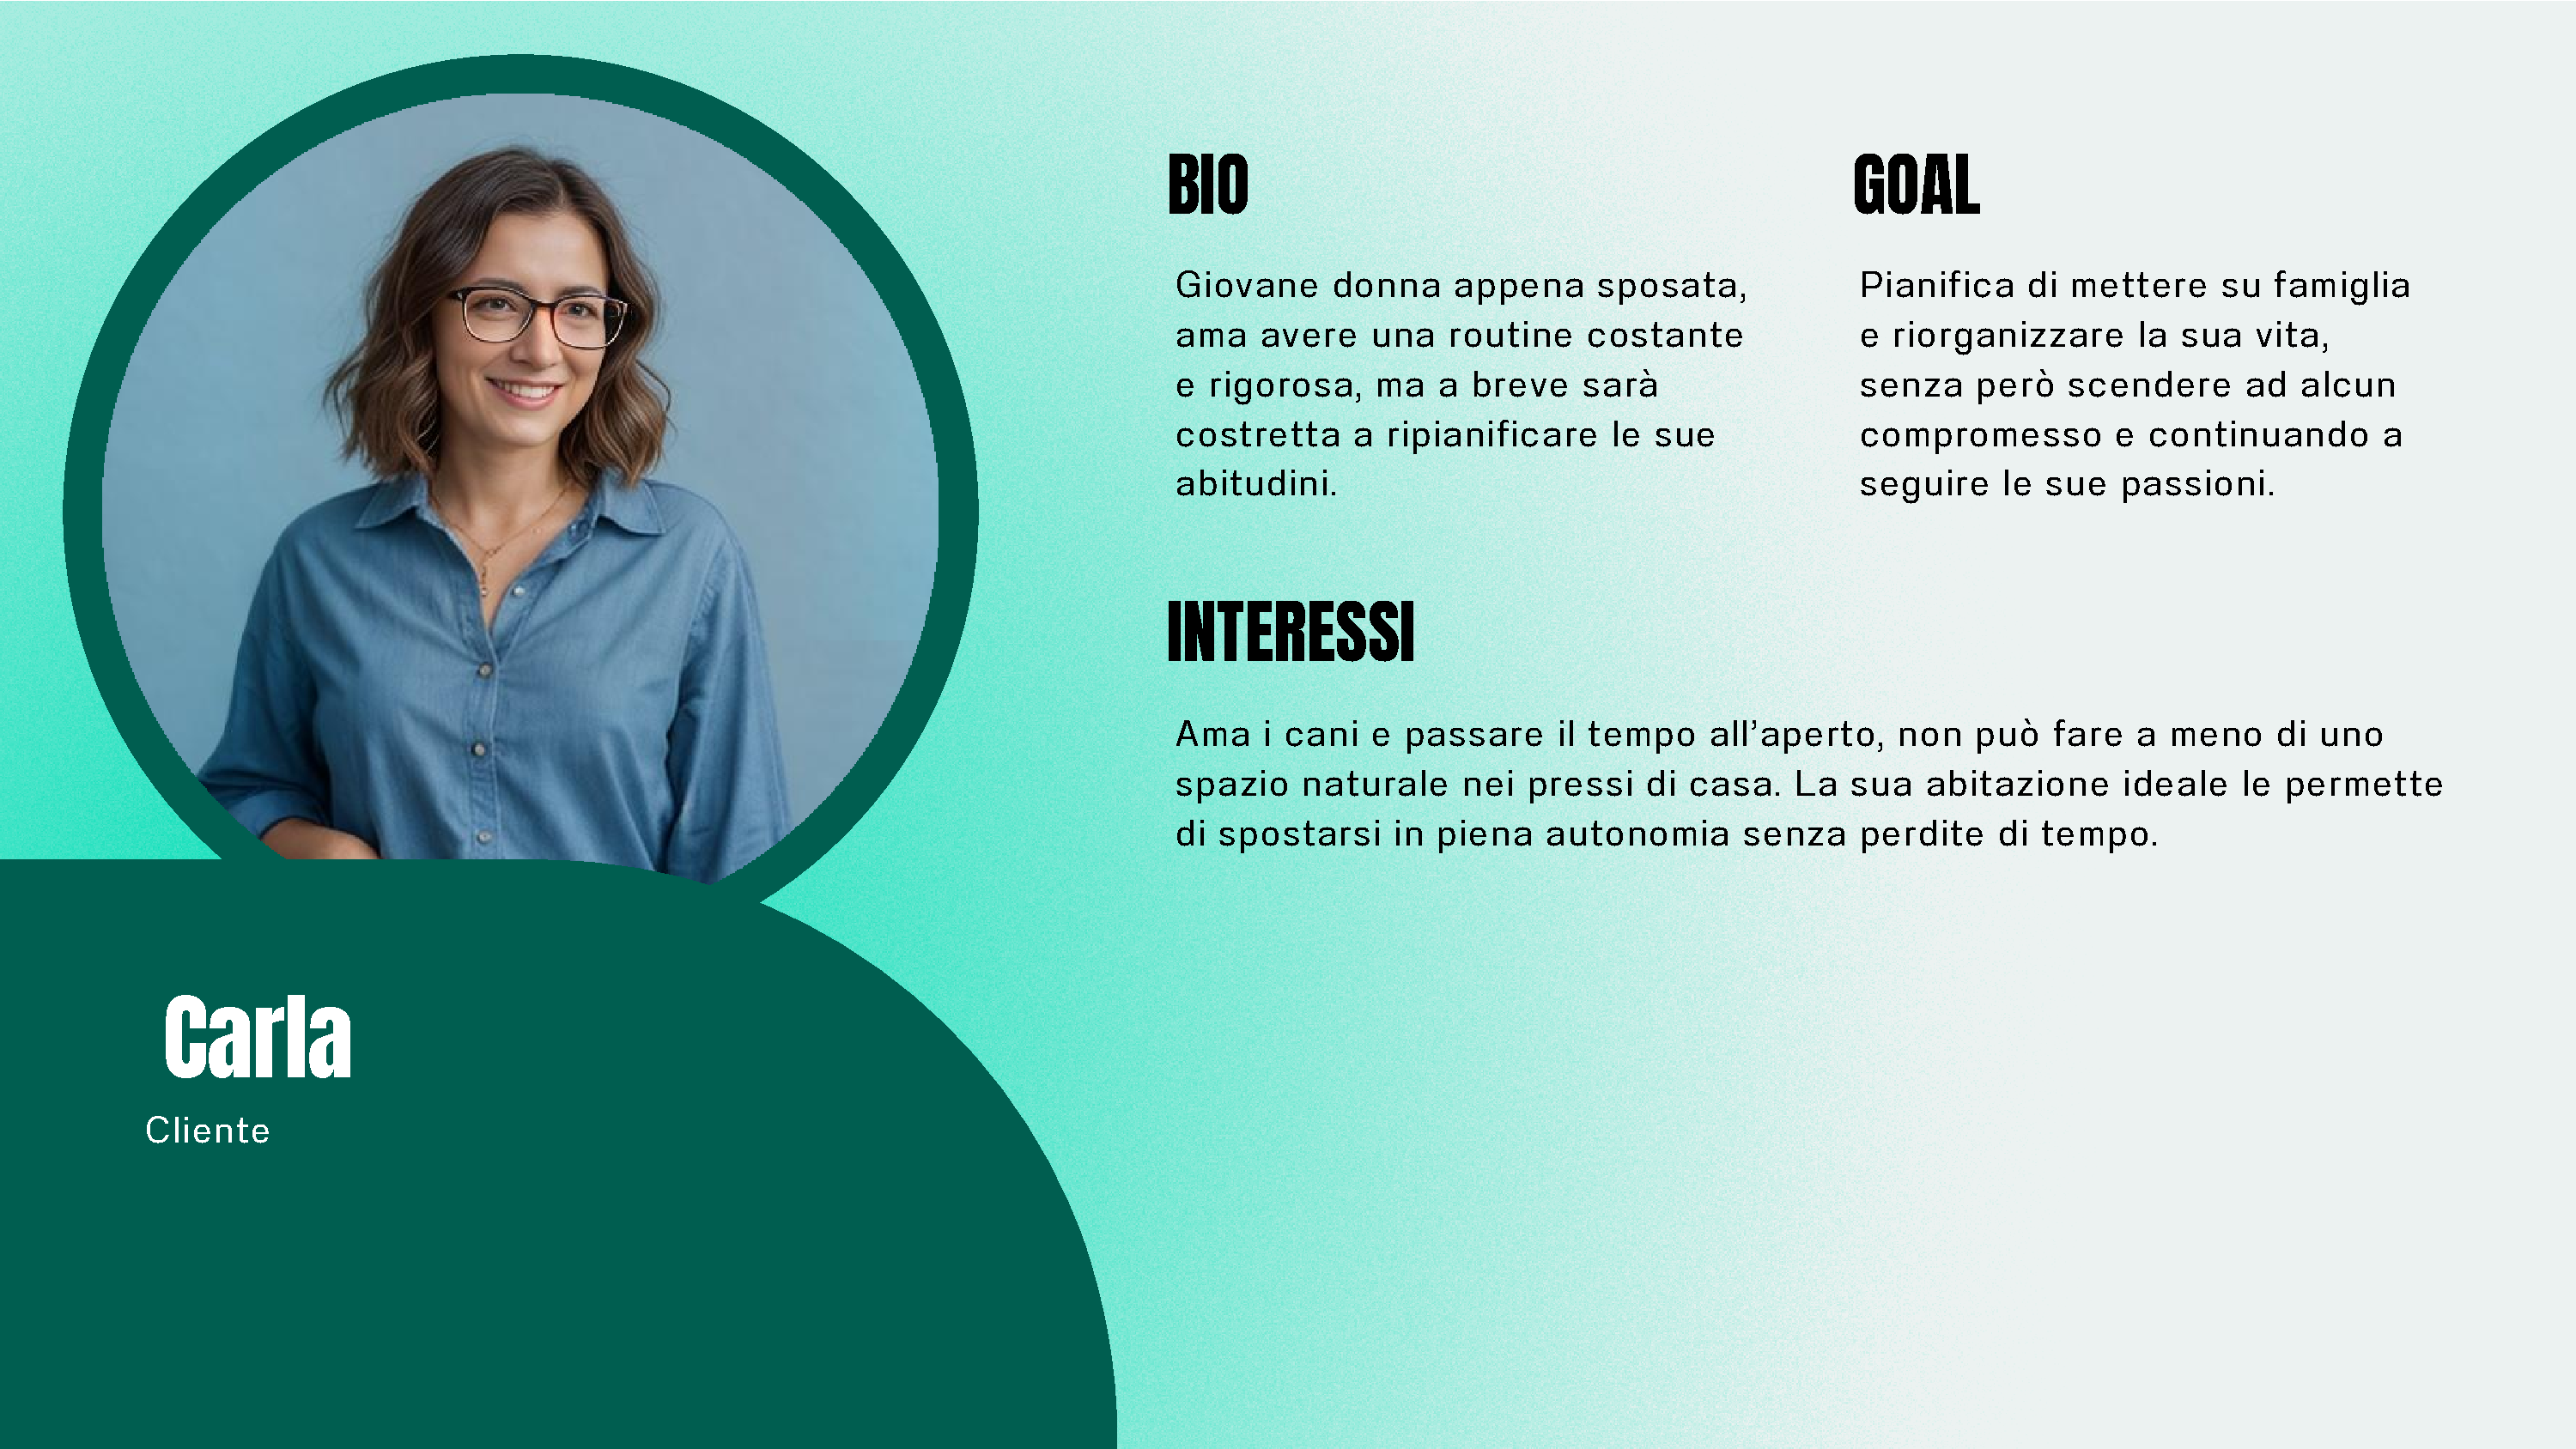
\includegraphics[width=\textwidth]{figures/youngclientPersona.pdf}
    \centering
    \caption{Esempio di \textit{Persona} rappresentativa di una cliente}
\end{figure}

\begin{figure}[!htb]
    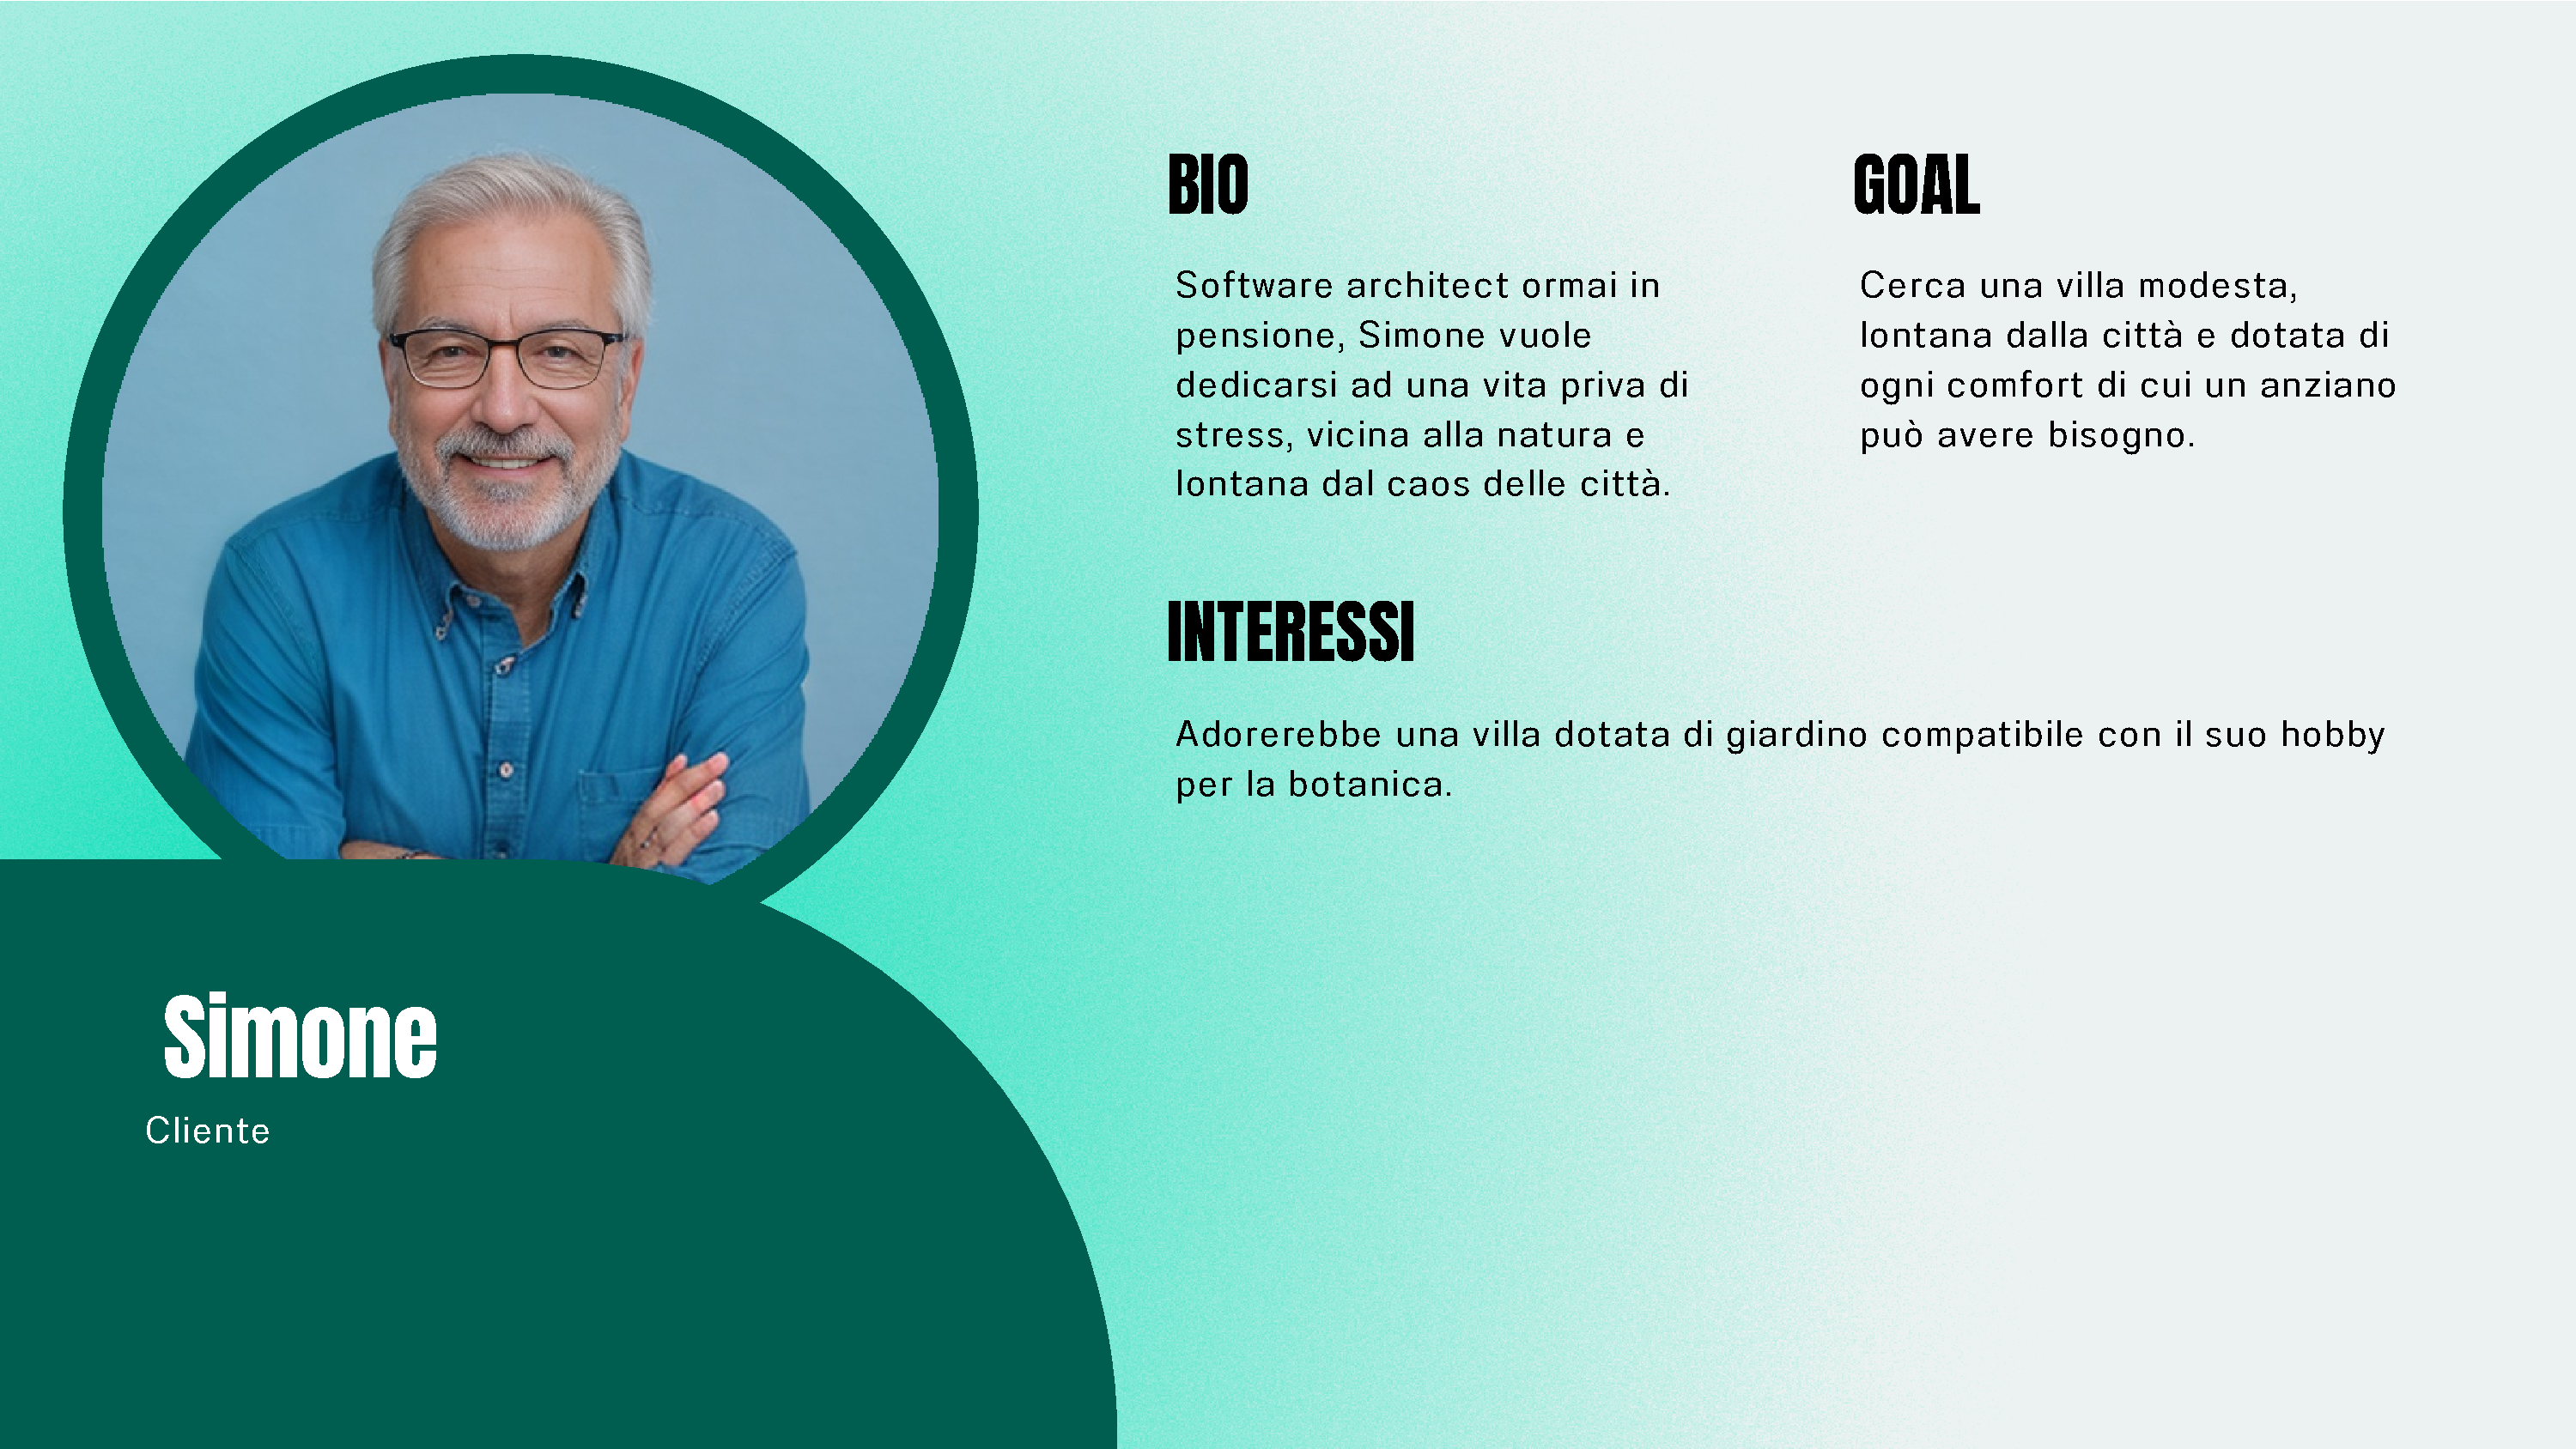
\includegraphics[width=\textwidth]{figures/oldclientPersona.pdf}
    \centering
    \caption{Esempio di \textit{Persona} rappresentativa di un cliente}
\end{figure}

\cleardoublepage
\subsection{Agenti immobiliari}
Un altro segmento significativo dell'utenza della piattaforma è rappresentato dagli agenti immobiliari, professionisti del settore, ingaggiati dalle agenzie che hanno scelto DietiEstates25. Dotati di una conoscenza approfondita degli immobili loro affidati, questi operatori interagiscono con i potenziali clienti attraverso il sistema di gestione delle offerte.

\begin{figure}[!htb]
    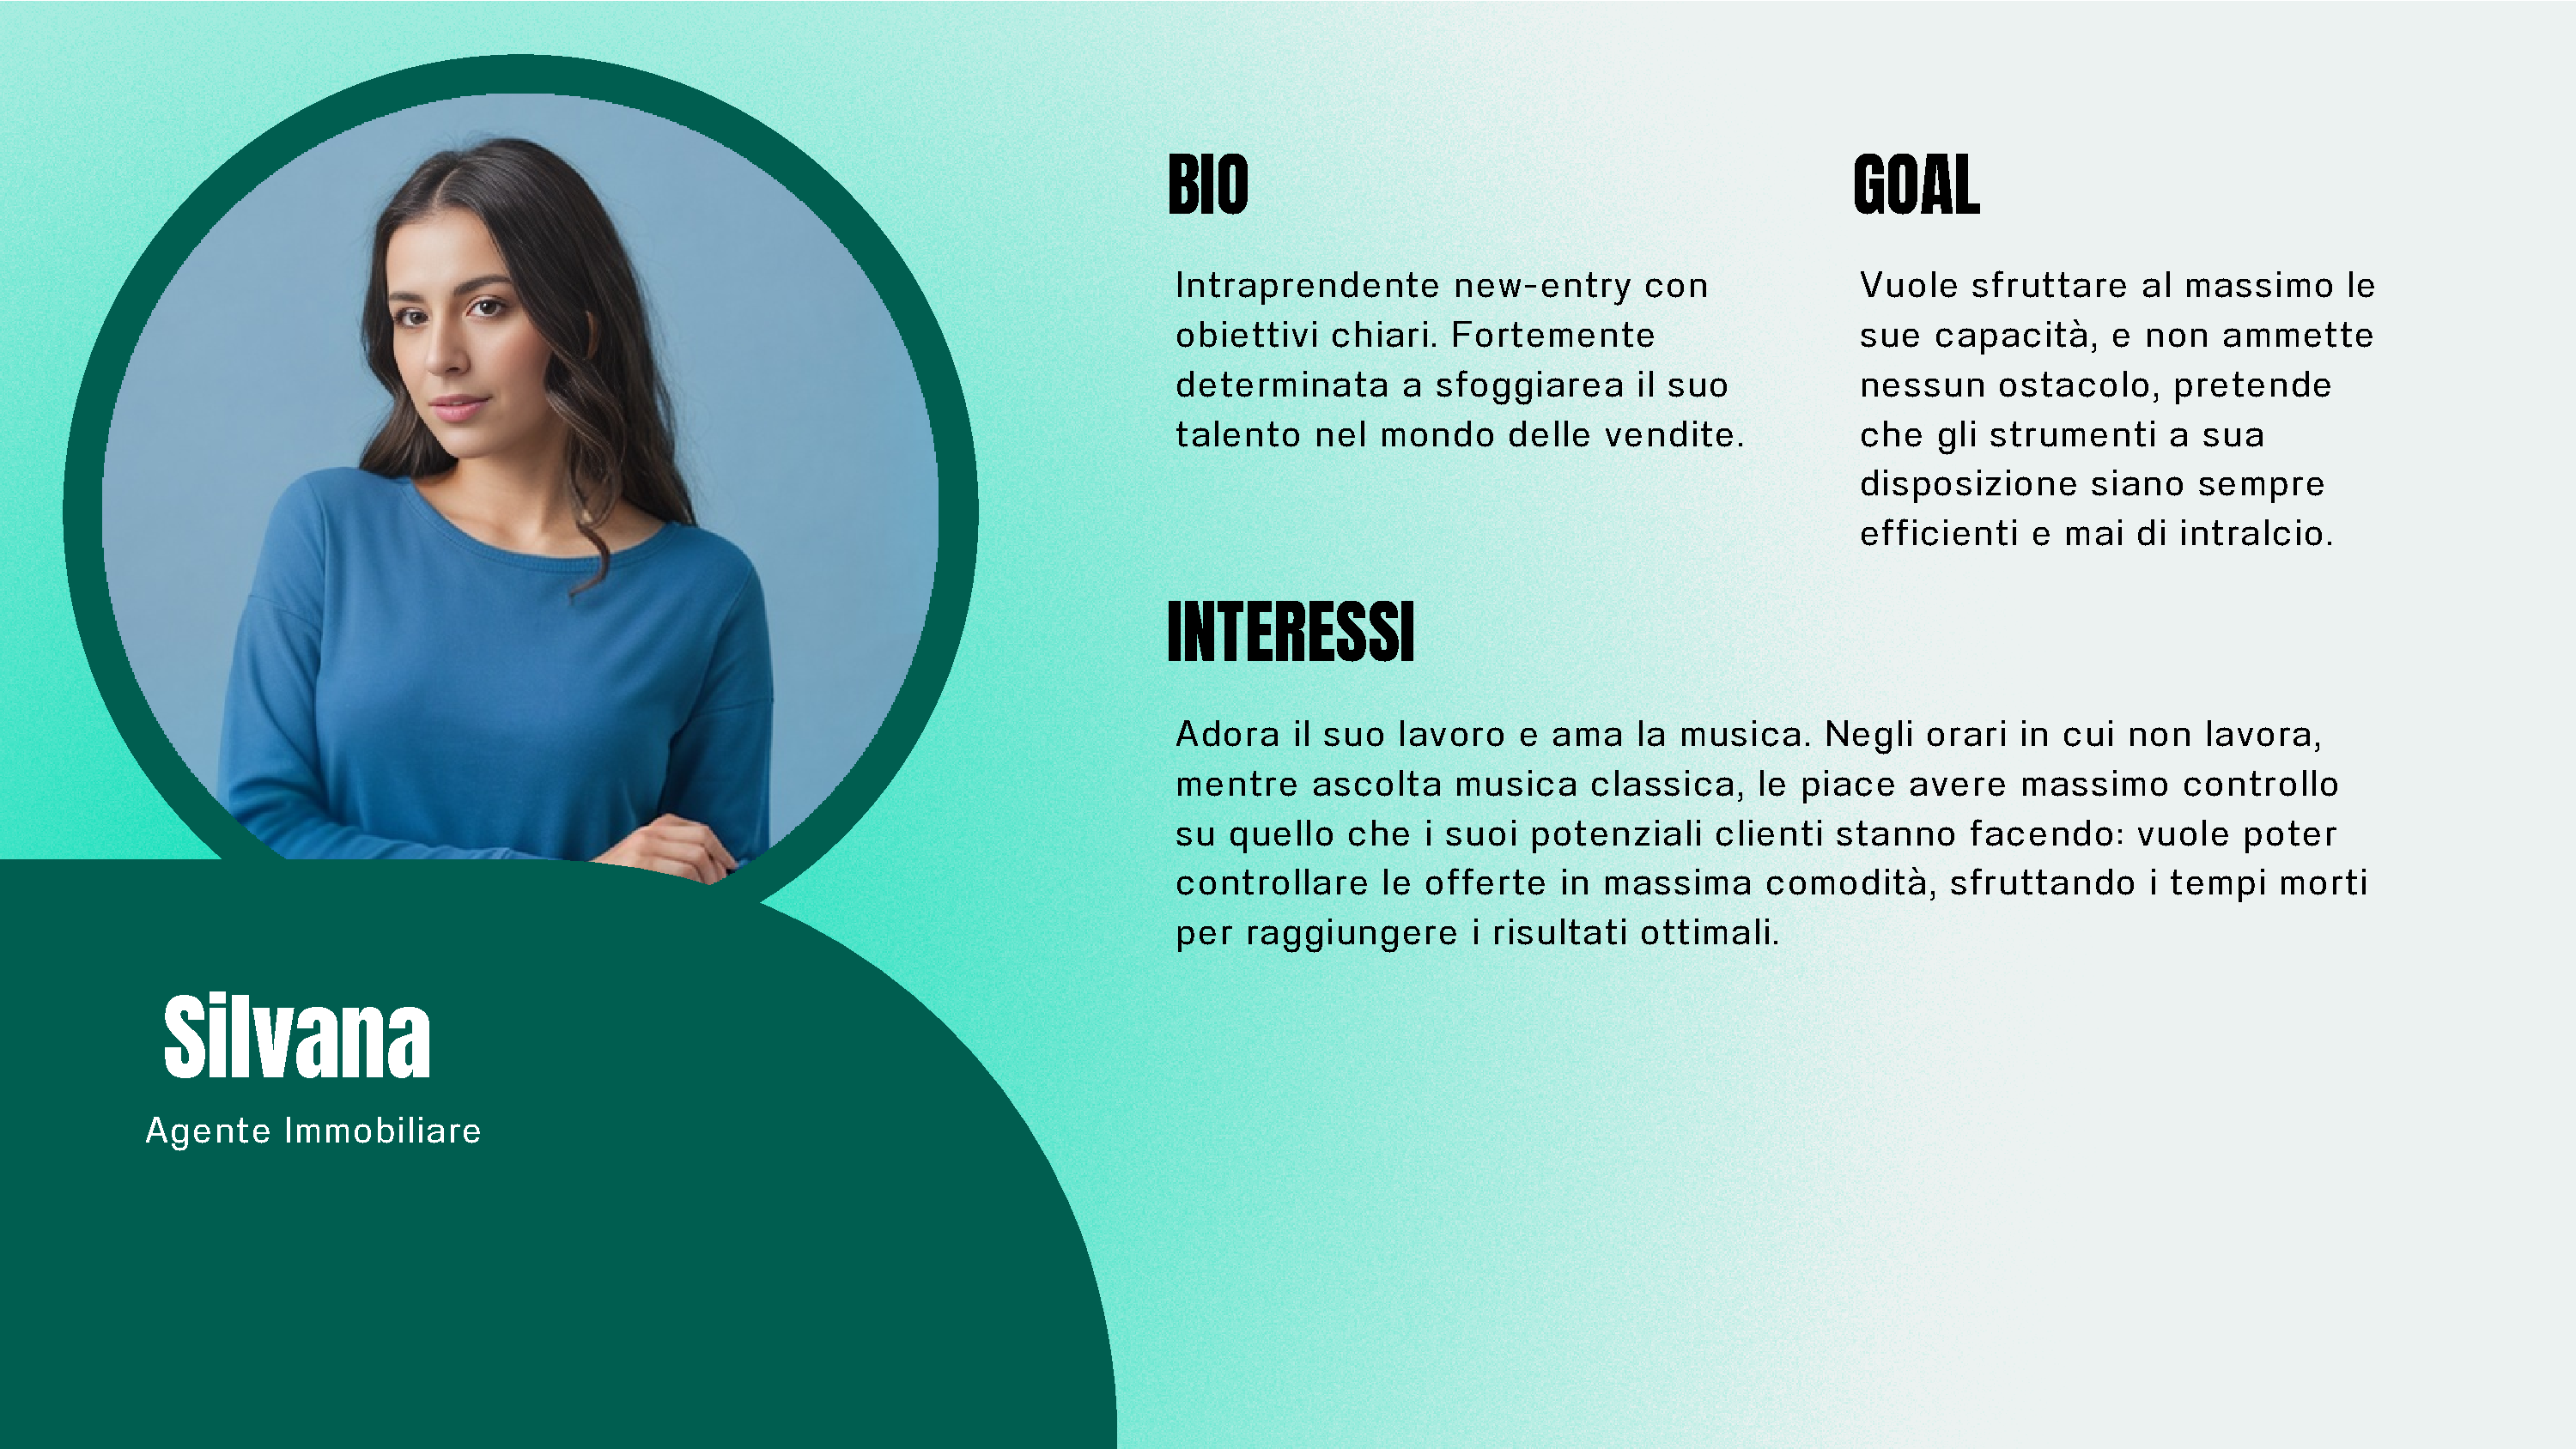
\includegraphics[width=\textwidth]{figures/reagentPersona.pdf}
    \centering
    \caption{Esempio di \textit{Persona} rappresentativa di un'agente immobiliare}
\end{figure}

\clearpage
\subsection{Amministratori}
La categoria con più privilegi è costituita dai gestori delle agenzie immobiliari. Dotati di accesso a funzionalità avanzate, hanno la possibilità di abilitare altri gestori e agenti immobiliari all'utilizzo della piattaforma.

\begin{figure}[!htb]
    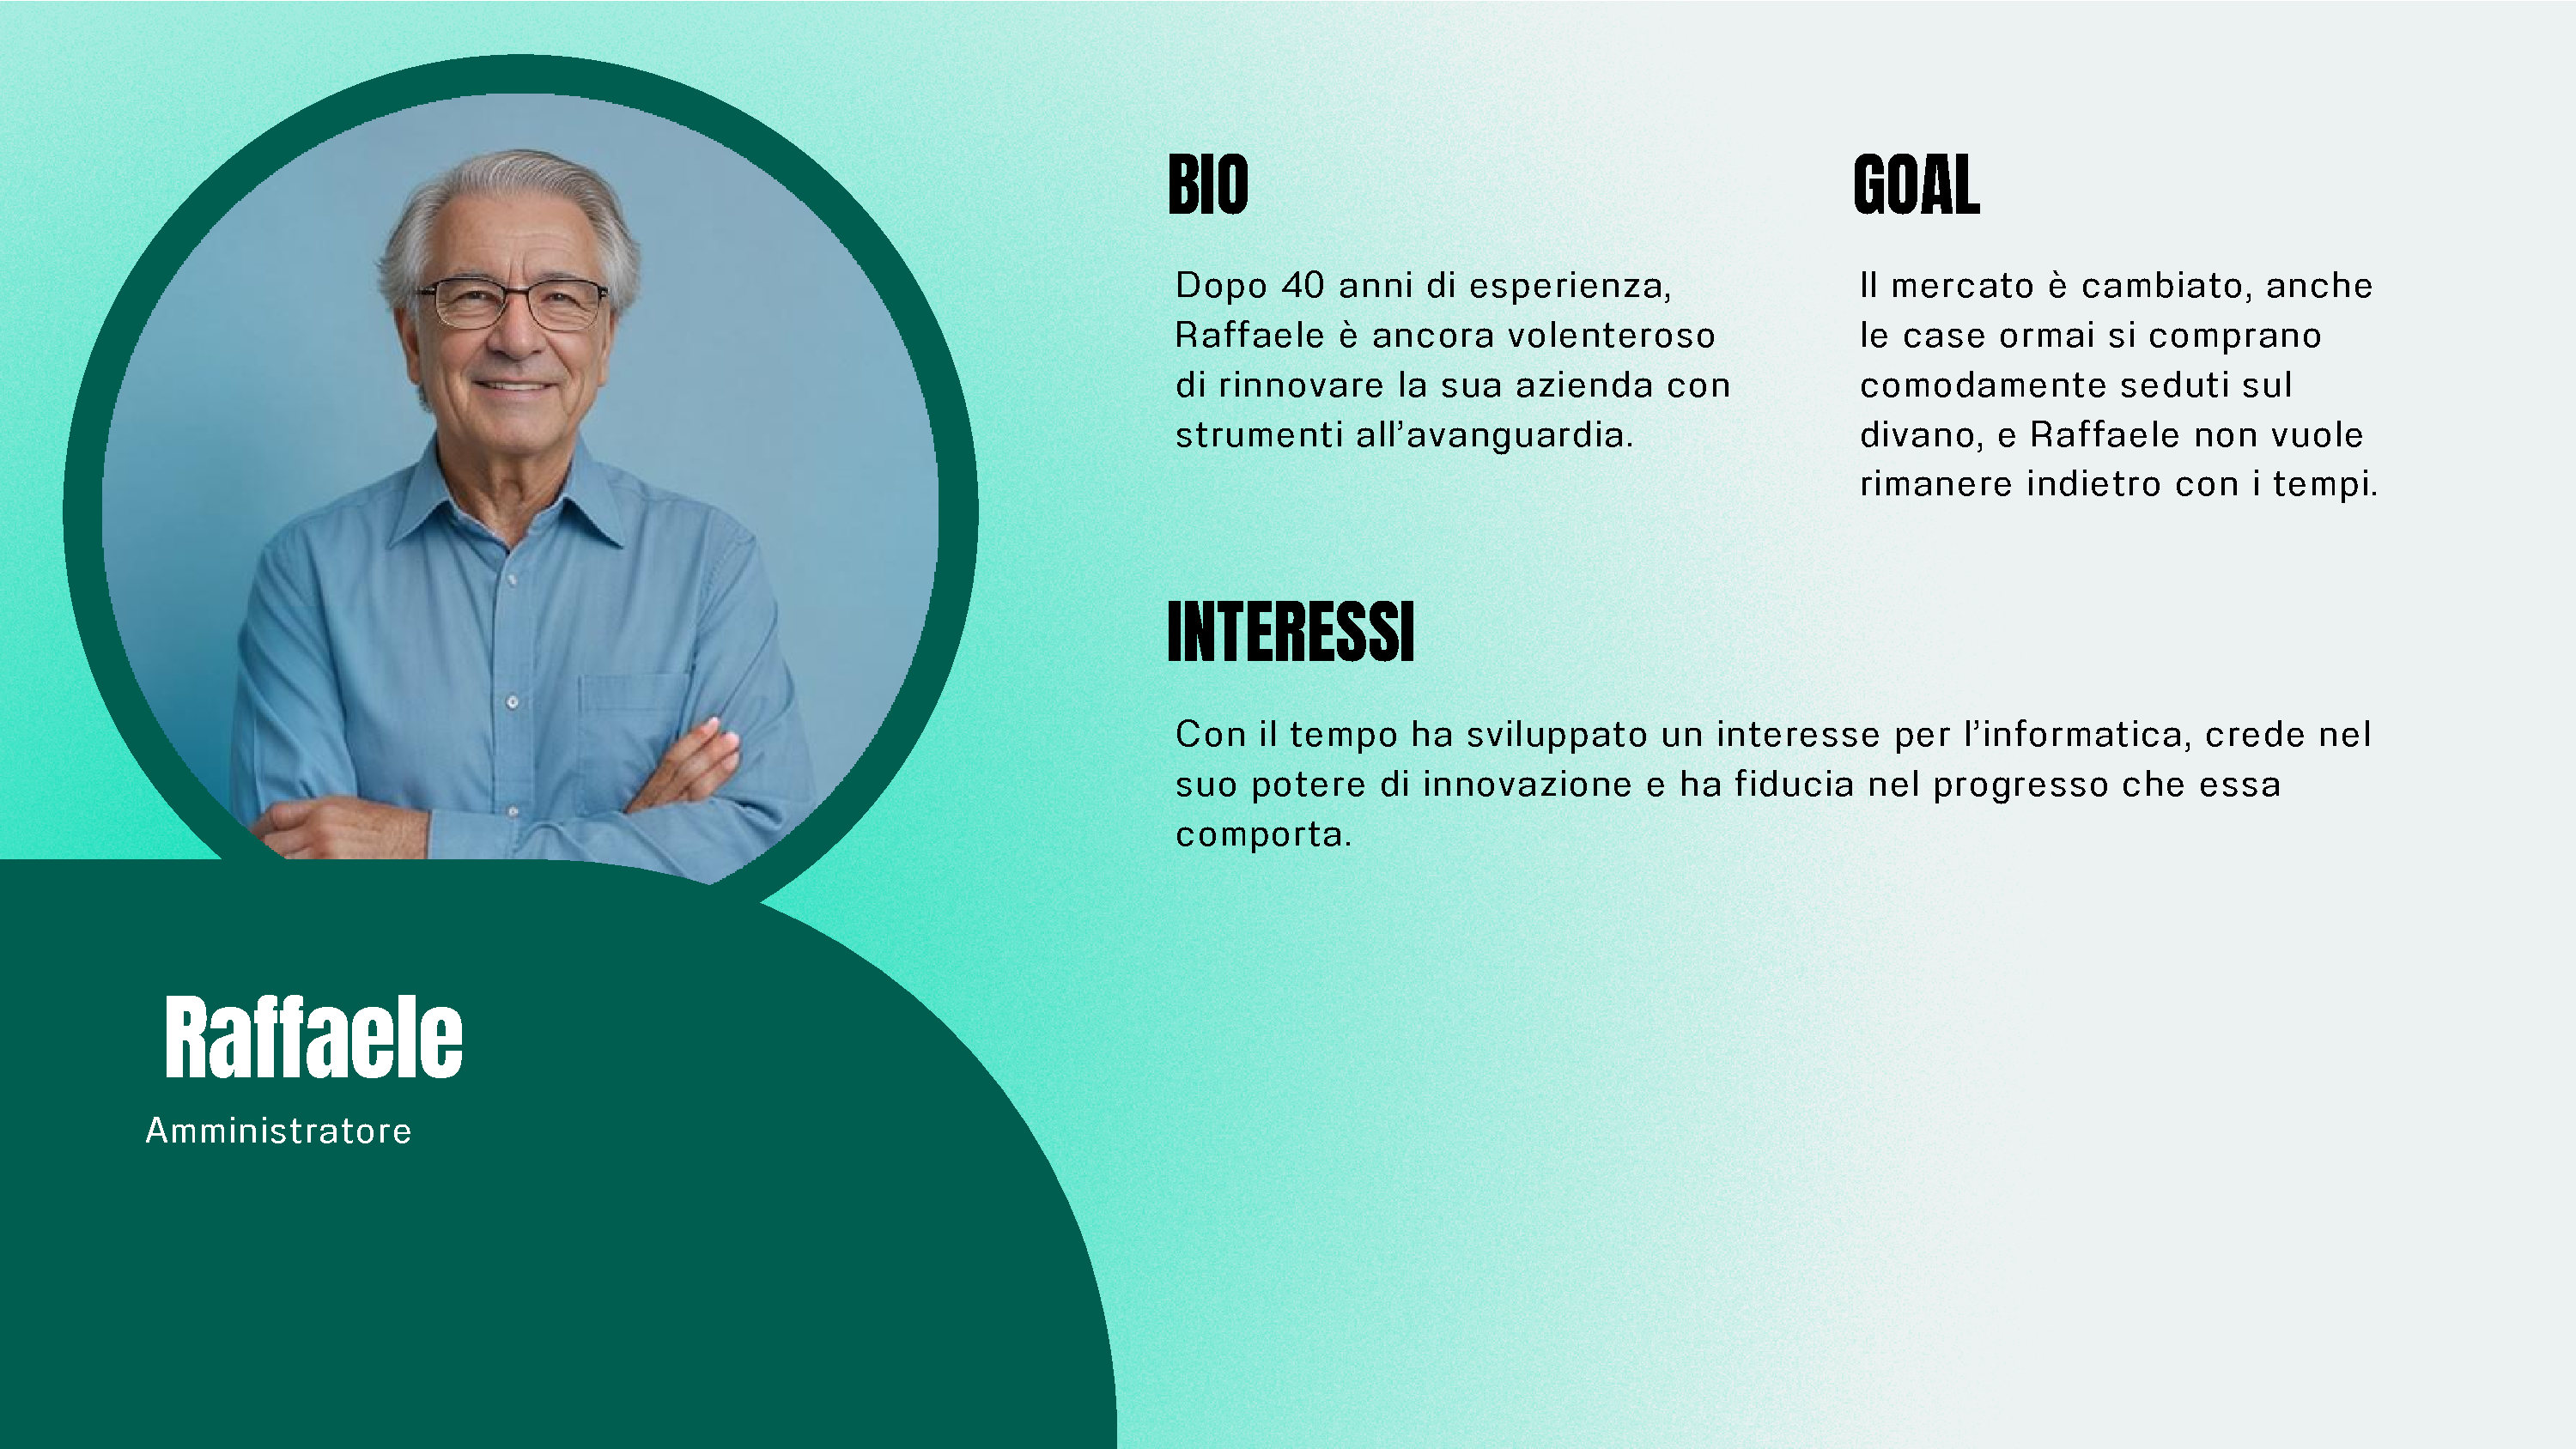
\includegraphics[width=\textwidth]{figures/adminPersona.pdf}
    \centering
    \caption{Esempio di \textit{Persona} rappresentativa di un amministratore}
\end{figure}

\section{Modellazione dei casi d'uso}
Individuati gli utenti target, si descrivono e schematizzano di seguito le funzionalità di DietiEstates25 e gli attori che ne prendono parte.

\subsection{Descrizione dei casi d'uso}
Gli \textbf{utenti} sono i principali attori della piattaforma, se ancora sono \textbf{non registrati} hanno la possiilità di:
\begin{itemize}
    \item \textbf{Registrarsi}: L'utente compila un form con le informazioni richieste per la creazione di un account e il sistema verifica la validità dei dati inseriti, creando il nuovo profilo.
\end{itemize}
Una volta \textbf{registrati}, possono:
\begin{itemize}
    \item \textbf{Autenticarsi}: L'utente inserisce le proprie credenziali nel form di login. Il sistema verifica la correttezza delle informazioni e, in caso positivo, concede l'accesso alla sua area riservata.
    \item \textbf{Ricercare immobili}: L'utente utilizza i filtri disponibili per cercare immobili. Il sistema elabora la richiesta e presenta i risultati corrispondenti ai parametri specificati.
    \item \textbf{Fare un'offerta su un immobile}: L'utente, selezionato un immobile, fa un'offerta per acquistarlo. Il sistema registra l'offerta.
    \item \textbf{Accettare un'offerta}: L'utente visualizza l'offerta ricevuta riguardo un immobile e la accetta. Il sistema aggiorna lo stato dell'offerta.
    \item \textbf{Rifiutare un'offerta}: L'utente esamina l'offerta ricevuta e la rifiuta. Il sistema aggiorna lo stato dell'offerta.
    \item \textbf{Fare una controproposta ad un'offerta}: L'utente, in risposta ad un'offerta ricevuta, formula una controproposta. Il sistema registra la controproposta.
    \item \textbf{Visualizzare storico offerte}: L'utente accede a una sezione dove può consultare l'elenco cronologico di tutte le offerte effettuate o ricevute, con i relativi dettagli.
\end{itemize}
Gli \textbf{agenti immobiliari}, oltre alle funzionalità degli \textbf{utenti}, possono:
\begin{itemize}
    \item \textbf{Caricare nuovi immobili}: L'agente immobiliare inserisce le immagini e le informazioni relative ad un immobile da vendere tramite un apposito form. Il sistema convalida le informazioni e pubblica l'annuncio sulla piattaforma.
    \item \textbf{Inserire un'offerta dall'esterno}: L'agente immobiliare registra manualmente un'offerta ricevuta all'esterno della piattaforma. Il sistema la registra nello storico.
\end{itemize}
Infine, i \textbf{gestori} hanno ancora ulteriori funzionalità, quali:
\begin{itemize}
    \item \textbf{Modificare la password di amministrazione}: Il gestore accede alle impostazioni dell'account e modifica la propria password. Il sistema verifica e salva la nuova password.
    \item \textbf{Creare account di supporto amministrazione}: Il gestore crea un nuovo account per nuovi amministratori. Il sistema genera le credenziali e imposta i permessi relativi.
    \item \textbf{Creare account per agenti immobiliari}: Il gestore crea un profilo per un nuovo agente immobiliare. Il sistema genera le credenziali e imposta i permessi relativi.
\end{itemize}

\subsection{Diagramma dei casi d'uso}
Tutti i casi d'uso individuati possono essere riassunti in un \textit{Use Case Diagram} UML\@.
%TODO inserire diagramma

\newpage
\section{Descrizione dei requisiti non funzionali e di dominio}
Descritti i requisiti funzionali di DietiEstates25, è necessario specificare i requisiti non funzionali e i requisiti di dominio, altrettanto importanti.

\subsection{Requisiti non funzionali}
I requisiti non funzionali fanno riferimento a caratteristiche del sistema come qualità, prestazioni, affidabilità e sicurezza.\\
Il Committente richiede che l'applicazione sia performante ed affidabile, attraverso cui gli utenti possano fruire delle funzionalità in modo intuitivo, rapido e piacevole. Tali richieste possono essere suddivise in più sezioni e tradotte nel seguente modo.
%TODO vedere come funziona l'applicazione e modificare di conseguenza
\subsubsection{Requisiti di performance}
La performance riguarda la capacità del sistema di elaborare e restituire informazioni in modo rapido, efficiente e fluido, garantendo tempi di risposta minimi. Si individuano e rispettano i seguenti requisiti:
\begin{itemize}
    \item L'applicazione deve garantire un caricamento delle pagine rapido e immediato, non superiore a TODO secondi.
    \item Il sistema deve restituire risultati alla ricerca di immobili in modo istantaneo, con un tempo massimo di TODO secondi.
    \item L'applicazione deve supportare contemporaneamente almeno TODO utenti senza cali di prestazioni.
    \item Il caricamento dedegli immobili deve avvenire velocemente, entro TODO secondi dalla conferma.
\end{itemize}
%TODO specifica che si è in condizioni normali di connettività internet etc
\subsubsection{Requisiti di affidabilità}
L'affidabilità misura la capacità del sistema di funzionare correttamente e continuativamente, gestendo eventuali errori senza perdita di dati o interruzione del servizio. Si individuano rispettano i seguenti requisiti:
\begin{itemize}
    \item L'applicazione deve garantire una disponibilità del servizio pressoché totale, con un uptime non inferiore al 99.TODO\%.
    \item In caso di malfunzionamento, il sistema deve ripristinarsi completamente in meno di TODO secondi.
    \item Il sistema deve gestire eventuali errori in modo trasparente, senza mai interrompere l'esperienza di navigazione dell'utente.
    \item L'applicazione deve possedere meccanismi di ripristino che consentano il recupero completo dei dati in caso di guasto.
\end{itemize}

\subsubsection{Requisiti di usabilità}
L'usabilità valuta la facilità di utilizzo dell'applicazione, misurando quanto l'interfaccia sia intuitiva, comprensibile e piacevole per l'utente finale. Si individuano rispettano i seguenti requisiti:
\begin{itemize}
    \item L'interfaccia utente deve consentire di completare qualsiasi azione principale con non più di TODO click.
    \item L'applicazione deve adattarsi perfettamente a schermi di qualsiasi dimensione, garantendo una visualizzazione ottimale.
    \item L'applicazione deve rispettare le linee guida di accessibilità WCAG livello AA\@.
    \item Il design deve garantire chiarezza assoluta di bottoni e menu, rendendone immediata la comprensione.
\end{itemize}

\subsubsection{Requisiti di sicurezza}
La sicurezza riguarda la protezione del sistema e dei dati degli utenti da manomissioni e violazioni della privacy. Si individuano rispettano i seguenti requisiti:
\begin{itemize}
    \item L'applicazione deve implementare una crittografia end-to-end che protegga totalmente i dati personali degli utenti.
    \item Il sistema deve possedere protezioni avanzate contro ogni tipo di attacco informatico.
    \item Il sistema deve essere totalmente conforme alle normative GDPR per la protezione dei dati personali.
    \item L'applicazione deve chiudere automaticamente le sessioni dopo TODO minuti di inattività per prevenire accessi non autorizzati.
\end{itemize}

\subsection{Requisiti di dominio}
I requisiti di dominio di DietiEstates25 sono specifiche derivanti dalla conoscenza del contesto operativo e professionale del settore immobiliare. Rappresentano l'insieme degli standard e delle normative tipiche del settore e vanno necessariamente incorporate nel sistema. Si individuano rispettano i seguenti requisiti:
\begin{itemize}
    \item Il sistema deve raccogliere esclusivamente i dati personali strettamente necessari, in conformità con l'Art. 5 del GDPR che prevede la minimizzazione dei dati.
    \item L'applicazione deve limitare la raccolta di informazioni solo agli elementi essenziali per la gestione dell'annuncio immobiliare.
    \item Deve essere implementata un'informativa privacy chiara e comprensibile, nel rispetto dell'Art. 13 del GDPR\@.
    \item L'applicazione deve implementare controlli di base per verificare la completezza e la coerenza dei dati inseriti negli annunci immobiliari.
    \item Il sistema fornirà linee guida chiare per la compilazione degli annunci, richiamando i principi di trasparenza previsti dal Codice Civile in materia di compravendita.
    \item Le credenziali di accesso saranno protette mediante tecniche di hashing, in linea con le best practice di sicurezza informatica.
    \item L'applicazione limiterà l'accesso ai dati personali, garantendo la protezione delle informazioni sensibili.
    \item Il sistema conserverà uno storico base delle versioni delle offerte, permettendone la tracciabilità. %TODO? permettere la tracciabilità delle modifiche degli ANNUNCI
\end{itemize}

\section{Glossario}
Sono di seguito definiti alcuni termini che sono stati utilizzati nel corso del capitolo.
%TODO fare riferimenti nel testo
\begin{itemize}
    \item \textbf{Mock-up}: realizzazione a scopo illustrativo di un sistema, senza le complete funzioni dell'originale.
    \item \textbf{UML} (\textit{Unified Modeling Language}): in ingegneria del software, linguaggio di modellazione e di specifica basato sul paradigma orientato agli oggetti.
    \item \textbf{Uptime}: intervallo di tempo in cui un sistema informatico è ininterrottamente acceso e correttamente funzionante.
\end{itemize}


\chapter{Progettazione del Sistema}
\chapter{Testing e Valutazione dell'Usabilità}
\end{document}